\begin{center}
ACKNOWLEDGMENTS
\end{center}
\setstretch{1.25}


I would like to thank several sources of funding I received throughout graduate school.
The William Webber Voyager Graduate Fellowship provided a welcome financial relief during the first two semesters that was especially important before the Graduate Workers Union wins to substantially increase salaries and tuition remission from the Graduate School for graduate workers.
I was also supported by teaching assistantships for three semesters, which provided some of the most humbling experiences during my time at New Mexico State University.
I was supported for three years by the National Science Foundation under grant NSF AST-2206096 which was awarded to release a public, open-source Monte Carlo simulation code for the community to simulate and test the sources from active galactic nuclei for LIGO/Virgo/Kagra gravitational wave detectors.
I also received a small amount of funding from several Department of Astronomy awards, namely the Pegasus Award, Rappaport Award, and Zia Award, and the Graduate school Outstanding Graduate Assistant Award.
Finally, my last semester was supported by the NMSU Spring Semester Graduate Assistantship Award.

First and foremost, I want to thank and acknowledge my advisor Dr. Wladimir Lyra. Wlad, I am so appreciative for all that you've done for me.
From the start, you took me on as your first Ph.D. student even though I said I was interested in AGN and galaxies not planets.
After asking around, you were able to connect me with the AGN channel folks in New York and we embarked on a quick project to blow up a star in a disk that would only take seven years!
On top of that, you nominated me for awards and scholarships practically looking under every planetesimal, pebble, and dust grain to find funding for me and my decidedly NOT planets research, though maybe there ARE planets in AGN disks.
I'm also grateful for your support beyond the research.
It got tough there for a while, and I'm uncertain I would have made it through without some of our breakfasts.
Also, a huge thanks to you and Adrienn for hosting all the delicious Brazilian barbeques and dinner parties for the group throughout the years.

I would also like to express thanks to my committee for their part in getting me here.
Dr. Moire Prescott, thanks for all of observational context that built my intuition for galaxies and AGN in the Galaxies I class.
I'll always remember when I mentioned in passing to Dr. Kristian Finlator that I had managed to successfully compile my supernova model on the Stampede 2 high performance computer using multiple nodes for the first time.
Your simple ``Congratulations! That's a great accomplishment." was unexpected and baffled me in the moment, since at the time it felt I had just done the barest of minimums, but it was most welcome and a compliment I didn't realize I needed to hear.
Dr. Michael Engelhardt, the general relativity will likely finally come in hand in the next phases of this work.

None of this work would have been possible without the hundreds (thousands?) of meetings with collaborators and research groups throughout the years.
Dr. Mordecai-Mark Mac Low, thanks for watching me live code and debug through video calls.
Your guidance was instrumental in kick-starting my hydrodynamics research and keeping me organized.
To Doctors Saavik Ford and Barry McKernan, you run incredible groups from TIDYNYC (Things In Disks Yo, NYC) to the McFAM.
Thank you for taking me into the fold.
I am so thankful I was able to know you all and be a part of something so fun!
I am especially grateful for the guidance I received from Ana Gabela that helped me publish my first academic research article.

My journey here started in 2012 while posted as a Marine Security Guard at the U.S. Embassy in Asunci\'on, Paraguay.
I had become fascinated with popular astronomy videos and started talking about them with everyone who would (and wouldn't) listen.
It was a small community, and eventually Ambassador James Thessin and Marcia Thessin caught wind.
Marcia came by Post One while I was on duty one day and asked if I wanted to come to the private Ambassador's quarters to have a video chat with their daugher Rachel Thessin who was an aerospace engineer and son-in-law Will Farr who was an astrophysicist to talk about getting into astronomy as a career.
I was humbled and flattered that they would invite a lowly Marine for such a thing and readily agreed.
At the appointed time, I arrived at the residence where Marcia walked me through the official quarters into the private residence and the small office where we connected with Rachel and Will.
They taught me about how to find papers on arXiv.org, look for schools with astronomy degrees, and focus my community college courses in preparation for mathematics and physics.
I had no idea how valuable that call would end up being, but I took their advice to heart and immersed myself in astronomy magazines, podcasts, and documentaries.
I even took pre-calculus for the second time at my next post in Kabul, Afghanistan where I had to travel in an up-armored vehicle while kitted up to another base in order to take proctored exams.
Perhaps needless to say, my mind wasn't all in it, and I had to take pre-calculus a third time in my life when I got to Columbia Univeristy.
But I passed and took accelerated calculus cources in order to start physics in my second year, sine I didn't want to spend longer than four hears in college.
So, thank you all James, Marcia, and Rachel Thessin and Will Farr for the roles each of you played in getting me started on my journey to astronomy back in Asunci\'on, Paraguay.
I've dedicated much of my efforts to paying this forward.

Thank you Dr. Nancy Chanover for inviting me to hide for the dog team practice back in Fall 2019.
I immediately fell in love with Mesilla Valley Search and Rescue.
Without the team, I would have missed out on so many unimaginable experiences with an awesome bunch.
I was able to see some magical places, and being involved with the cause kept me sane when things got tough.
So that others may live.

To my many friends, 
Issiah Astorga and Araceli Hernandez, I'm looking forward to the time when we can all camp in peace, maybe at Cosmic Campground.
I know it will happen one day.
To my brothers and sister from Kabul, it's been such a blessing and lifeline to reconnect with everyone.
For Rod.
And, it's been so great having another veteran around, Jessica Klusmeyer.
I'm glad that will continue.
I've had awesome office mates throughout: Matt Varakian, Alec Herczeg, Cristo Sanchez, and Samir Kusmic.
If you're reading this Kevin Brooks, let me know when you decide to abandon the Sun and start studying a \emph{real} astrophysical object.
To the Q, Hannah Gallamore, Mark Croom, and Audrey Dijeau, the continuum has expanded, but it just means we've evolved into an even higher state of being.
Ezra Huscher, your curiosity and willingness to entertain all of my crazy ideas and musings has inspired me to flex that creativity muscle again -- just you wait.
Dr. Ali Hyder, you were the first person I met at the department (after getting my key from Ofelia I suppose).
Without you, I may have given up on hydrodynamics early in the beginning, but it was our deep conversations about the awesome things we learned and could do with that knowledge that kept me motivated when I was lost in the sauce.
Dr. Priscilla Holguin Luna, you radiate such a unique perspective on life and the world.
From the very first day when we met on that first Zoom call, you have actively challenged me to be a better human and left a truly timeless imprint on my soul.
``Even when you're down..."

My family has been the bedrock of this marathon pursuit.
Unca Bob Cook, as the nearest extended family for so many years growing up, you have been a constant source of levity and encouragement that I would be lesser without.
I never considered myself a writer, but Garret Ray, our conversations about the challenges of writing and ways you overcome them and now have two published novels really helped get me through the toughest hurdles of getting words on the page.
Looking forward to reading what we both write in the future!
Wow, what an unexpected surprise to find out I have another cousin going to NMSU that I've never met.
Anna Dykeman, you're truly one of the best, and I think we need to get another beer together soon. 

Mom and Dad, when things were at their worst, and when it all felt impossible you'd say, ``We know you can do it. You're doing amazing things."
I could feel that you \emph{knew} that to be true, and I could hold that in my core.
I'm so thankful you're my parents.
Madison Snarr, if laughter was a force you'd be matriarch of the Universe.
I don't know how it's possible to laugh more when you're around, but let's try.
Brother, you inspire me at every turn, and I am always thinking about how Mitch would take on a difficult situation in stride and turn it into something motivating.
Sometimes if felt like that workout regimen you had me on to prepare for the Bataan Memorial Death March was taking time away from this dissertation, but in reality it gave me a consistent framework on which to base my writing and preparation while boosting my mental fortitude in magnitudes.

Pluto, you're simply the best girl and best full-sized planet.
Every day you're up to something new that keeps life interesting.
Maybe after finishing this Ph.D. I can sleep as much as you.
Do you ... wanna go ... camping?

And finally, Massi.
I simply could not have done this without you.
Thank you for waiting for me to go back to school all these years.
I'm so excited for what the next phase of life brings.
I'm more excited to see it with you.
\raisebox{-0.7ex}{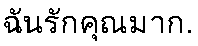
\includegraphics[height=2.75ex]{intro_figs/thai.pdf}}
